% Options for packages loaded elsewhere
\PassOptionsToPackage{unicode}{hyperref}
\PassOptionsToPackage{hyphens}{url}
\PassOptionsToPackage{dvipsnames,svgnames,x11names}{xcolor}
%
\documentclass[
  10pt,
]{article}
\usepackage{amsmath,amssymb}
\usepackage{iftex}
\ifPDFTeX
  \usepackage[T1]{fontenc}
  \usepackage[utf8]{inputenc}
  \usepackage{textcomp} % provide euro and other symbols
\else % if luatex or xetex
  \usepackage{unicode-math} % this also loads fontspec
  \defaultfontfeatures{Scale=MatchLowercase}
  \defaultfontfeatures[\rmfamily]{Ligatures=TeX,Scale=1}
\fi
\usepackage[]{libertine}
\ifPDFTeX\else
  % xetex/luatex font selection
\fi
% Use upquote if available, for straight quotes in verbatim environments
\IfFileExists{upquote.sty}{\usepackage{upquote}}{}
\IfFileExists{microtype.sty}{% use microtype if available
  \usepackage[]{microtype}
  \UseMicrotypeSet[protrusion]{basicmath} % disable protrusion for tt fonts
}{}
\makeatletter
\@ifundefined{KOMAClassName}{% if non-KOMA class
  \IfFileExists{parskip.sty}{%
    \usepackage{parskip}
  }{% else
    \setlength{\parindent}{0pt}
    \setlength{\parskip}{6pt plus 2pt minus 1pt}}
}{% if KOMA class
  \KOMAoptions{parskip=half}}
\makeatother
\usepackage{xcolor}
\usepackage[margin=2.4cm]{geometry}
\usepackage{longtable,booktabs,array}
\usepackage{calc} % for calculating minipage widths
% Correct order of tables after \paragraph or \subparagraph
\usepackage{etoolbox}
\makeatletter
\patchcmd\longtable{\par}{\if@noskipsec\mbox{}\fi\par}{}{}
\makeatother
% Allow footnotes in longtable head/foot
\IfFileExists{footnotehyper.sty}{\usepackage{footnotehyper}}{\usepackage{footnote}}
\makesavenoteenv{longtable}
\usepackage{graphicx}
\makeatletter
\def\maxwidth{\ifdim\Gin@nat@width>\linewidth\linewidth\else\Gin@nat@width\fi}
\def\maxheight{\ifdim\Gin@nat@height>\textheight\textheight\else\Gin@nat@height\fi}
\makeatother
% Scale images if necessary, so that they will not overflow the page
% margins by default, and it is still possible to overwrite the defaults
% using explicit options in \includegraphics[width, height, ...]{}
\setkeys{Gin}{width=\maxwidth,height=\maxheight,keepaspectratio}
% Set default figure placement to htbp
\makeatletter
\def\fps@figure{htbp}
\makeatother
\setlength{\emergencystretch}{3em} % prevent overfull lines
\providecommand{\tightlist}{%
  \setlength{\itemsep}{0pt}\setlength{\parskip}{0pt}}
\setcounter{secnumdepth}{5}

\usepackage{algorithm}
\usepackage{algpseudocode}
\usepackage[font=small,labelfont=bf]{caption}
\usepackage{xurl}
\usepackage{fancyhdr}
\pagestyle{fancy}\fancyhf{}\renewcommand{\headrulewidth}{0pt}
\fancyhead[C]{\footnotesize\itshape Query-Efficient Black-Box Knowledge Distillation from Pure Noise}
\fancyfoot[C]{\thepage}
\setlength{\LTpre}{6pt}\setlength{\LTpost}{6pt}
\ifLuaTeX
  \usepackage{selnolig}  % disable illegal ligatures
\fi
\IfFileExists{bookmark.sty}{\usepackage{bookmark}}{\usepackage{hyperref}}
\IfFileExists{xurl.sty}{\usepackage{xurl}}{} % add URL line breaks if available
\urlstyle{same}
\hypersetup{
  pdftitle={Query-Efficient Black-Box Knowledge Distillation from Pure Noise: Student-Side Projected Gradient Ascent and Student-Guided Query Selection},
  pdfauthor={Suneel 2023UG000150 2023suneel@vidyashilp.edu.in; Shaik Sameer Roshan 2024UG100001 2023shaiksameer.roshan@vidyashilp.edu.in; S Venkata Prasanna Bhargava 2023UG000129 2023venkataprasanna.bhargava@vidyashilp.edu.in; Rajesh 2023UG000184 2023rajesh.s@vidyashilp.edu.in},
  colorlinks=true,
  linkcolor={blue},
  filecolor={Maroon},
  citecolor={Blue},
  urlcolor={blue},
  pdfcreator={LaTeX via pandoc}}

\title{Query-Efficient Black-Box Knowledge Distillation from Pure Noise:
Student-Side Projected Gradient Ascent and Student-Guided Query
Selection}
\usepackage{etoolbox}
\makeatletter
\providecommand{\subtitle}[1]{% add subtitle to \maketitle
  \apptocmd{\@title}{\par {\large #1 \par}}{}{}
}
\makeatother
\subtitle{ATDL Course Project --- Final Report}
\author{\textbf{Suneel}\\
2023UG000150\\
2023suneel@vidyashilp.edu.in \and \textbf{Shaik Sameer Roshan}\\
2024UG100001\\
2023shaiksameer.roshan@vidyashilp.edu.in \and \textbf{S Venkata Prasanna
Bhargava}\\
2023UG000129\\
2023venkataprasanna.bhargava@vidyashilp.edu.in \and \textbf{Rajesh}\\
2023UG000184\\
2023rajesh.s@vidyashilp.edu.in}
\date{Vidyashilp University, 23 November 2026}

\begin{document}
\maketitle
\begin{abstract}
We study black-box, data-free knowledge distillation on CIFAR-100 under
strict constraints. The teacher, a ResNet-34 with 82.18\% test accuracy,
can only be queried. It reveals either its full probability vector (soft
labels) or only its arg-max class (hard labels). It may only be shown
random-noise images, and at most 250,000 teacher queries are allowed;
queries to our own students are free.

Following the design proposed by our supervisor, a ResNet-18 student is
distilled from teacher-labelled noise. It is then refined with Projected
Gradient Ascent (PGA) performed on the student: synthetic images are
driven towards a target class at a prescribed confidence, while a
KL-divergence term in the student's softmax space keeps images of the
same class far apart. These synthetic images are never shown to the
teacher.

We extend this design with student-guided query selection. An ensemble
of three students scores a pool of 1.6 million free noise images. The
teacher budget is spent over four active-learning rounds on images
chosen to be class-balanced and to maximise the students' disagreement.

With an identical budget of 250K queries, the proposed method improves
the single-student accuracy from 35.0\% to 41.4 \(\pm\) 0.6\% with soft
labels and from 24.5\% to 30.5 \(\pm\) 1.0\% with hard labels (3 seeds).
It surpasses a baseline that is given twice the budget. A comprehensive
ablation study attributes the gain to class-balanced,
disagreement-driven selection. The PGA refinement helps a single student
by up to 1.4 points but is subsumed once selection is used. We show
quantitatively that the diversity term does spread same-class samples
apart in the student's softmax space (mean pairwise symmetric KL 0.75
\(\to\) 3.47). We explain why this does not translate into accuracy, and
analyse the limits of distillation from pure noise.

Code, configurations and per-run results are available at
https://github.com/prxshu05/ATDL-FINAL.
\end{abstract}

\hypertarget{introduction}{%
\section{Introduction}\label{introduction}}

Machine-learning models are increasingly deployed behind application
programming interfaces (APIs): a user submits an input and receives a
prediction, but has no access to the model's parameters, gradients or
training data. \emph{Black-box knowledge distillation} (KD) asks how
well a new model, the \emph{student}, can be trained solely by querying
such a \emph{teacher}. The question matters from two complementary
perspectives:

\begin{itemize}
\tightlist
\item
  \textbf{Model compression.} It enables compact models to be derived
  from proprietary ones when the original training data is private.
\item
  \textbf{Security.} It is the mechanism behind \emph{model-stealing}
  attacks, so the number of queries needed to replicate a model directly
  measures how much protection a query limit offers.
\end{itemize}

The most demanding variant is \emph{data-free} distillation. Here no
natural images are available, so the student must learn from synthetic
inputs, and every teacher answer has a monetary or rate-limit cost. Most
existing methods, such as DFME {[}3{]}, IDEAL {[}6{]}, DisGUIDE {[}7{]}
and CaBaGE {[}10{]}, train an image generator against the student (and
sometimes the teacher) and consume between two and several tens of
millions of queries. They also send the teacher images that were
explicitly optimised for the attack.

This project follows a stricter protocol proposed by our supervisor:

\begin{enumerate}
\def\labelenumi{\arabic{enumi}.}
\tightlist
\item
  The teacher is a black box.
\item
  No natural training data is used.
\item
  The teacher is only ever shown random noise.
\item
  At most 250K teacher queries are allowed.
\item
  All image optimisation (PGA) is performed on the student, with a
  diversity criterion defined in the student's softmax space.
\end{enumerate}

Because the teacher never sees optimised images, all intelligence on the
teacher side must lie in \emph{which} noise images are queried.

\textbf{Contributions.}

\begin{itemize}
\tightlist
\item
  \textbf{A faithful implementation of the supervisor's method.} It
  covers the noise seed, teacher labelling, soft-label (KL) and
  hard-label (CE) distillation, and student-side PGA with a symmetric-KL
  diversity objective over the non-target softmax. The query budget is
  enforced in code.
\item
  \textbf{Student-guided, class-balanced query selection.} A
  three-student ensemble scores free noise with a standardised
  combination of class confidence and Jensen--Shannon disagreement. The
  budget is allocated over four active-learning rounds with
  deficit-driven class quotas. At equal budget this improves accuracy by
  about 6 points for both label types.
\item
  \textbf{A systematic empirical study.} It comprises 40 training runs:
  3 seeds for the main configurations, a budget sweep from 50K to 500K
  queries, 9 ablations, per-class and information-theoretic analyses,
  and a direct visualisation of the effect of the diversity term.
\item
  \textbf{A careful comparison with the literature,} together with a
  discussion of the limitations of noise-only distillation.
\end{itemize}

\hypertarget{related-work}{%
\section{Related Work}\label{related-work}}

\textbf{Knowledge distillation and data-free KD.} Hinton et al.~{[}1{]}
introduced distillation with temperature-softened teacher probabilities.
Data-free methods synthesise their own training inputs: DAFL {[}21{]}
trains a generator whose outputs the teacher classifies confidently,
DeepInversion {[}16{]} matches the batch-normalisation statistics stored
in the teacher, and CMI {[}22{]} adds a contrastive term to diversify
the synthesised images. These methods require white-box access to
gradients and internal statistics and are therefore inapplicable here.
Two of their ideas nonetheless motivate the present design: optimising
images towards a class, and explicitly enforcing diversity among
synthetic samples.

\textbf{Black-box model stealing with soft labels.} Knockoff Nets
{[}23{]} query the teacher with natural images from a surrogate dataset,
which requires real data. DFME {[}3{]} and MAZE {[}4{]} train a
generator to maximise the teacher--student discrepancy and estimate the
teacher's gradient by zeroth-order finite differences. They require
20--30M queries even on CIFAR-10. CaBaGE {[}10{]} combines a generator
ensemble with class-balanced, difficulty-weighted replay and selective
querying. It recovers 75.96\% of a 77.52\% teacher on CIFAR-100 with
millions of queries.

\textbf{Black-box model stealing with hard labels.} Hard labels convey
at most \(\log_2 100 \approx 6.6\) bits per query, which makes the
problem substantially harder:

\begin{itemize}
\tightlist
\item
  ZSDB3KD {[}2{]} reconstructs soft labels from distances to the
  teacher's decision boundaries, at a large query cost.
\item
  DFMS-HL {[}5{]} trains a generator with a class-diversity loss (about
  10M queries).
\item
  IDEAL {[}6{]} trains the generator only against the student and labels
  each synthetic image once, reaching 36.96\% on CIFAR-100 with 2M
  queries.
\item
  DisGUIDE {[}7{]} uses two students and seeks inputs on which they
  disagree. Dual-student variants {[}8{]} report failures on CIFAR-100
  caused by class imbalance.
\item
  MGCT {[}24{]} and stabilised DFME {[}25{]} add multiple generators and
  class-balance constraints.
\item
  DFHL-RS {[}9{]} extracts accuracy and robustness from a robust teacher
  with tens of millions of queries.
\item
  Attacks based on diffusion models {[}12{]} reach about 57--60\% with
  150K queries, but their inputs carry prior knowledge of natural
  objects.
\end{itemize}

\textbf{Image priors and noise.} Closest to our setting is DIP-KD
{[}11{]}. It queries a hard-label teacher only with fixed synthetic
priors (hierarchical noise, non-linear warps and semantic CutMix) and
adds contrastive learning and a ``primer'' student. It reports 52.85\%
on CIFAR-100 with 100K images. Baradad et al.~{[}15{]} showed that
procedural noise with natural-image statistics can pre-train useful
representations, and that the diversity of the noise is critical.

\textbf{Query selection and class imbalance.} ActiveThief {[}13{]}
selects pool samples for labelling by student uncertainty. A follow-up
{[}14{]} identifies the resulting class imbalance as a major failure
mode and corrects it by re-weighting and rare-class sampling. Our
stage-B selection follows this line, but operates on a pool of
\emph{free noise} rather than natural images.

\textbf{Projected gradient ascent.} ZOPGA-KD {[}17{]} synthesises
class-targeted images by PGA on the \emph{teacher}, using zeroth-order
gradient estimates that each cost many queries. The supervisor's variant
moves PGA to the \emph{student}, whose gradients are exact and free, and
adds a diversity term defined in the student's softmax space.

\begin{longtable}[]{@{}
  >{\raggedright\arraybackslash}p{(\columnwidth - 8\tabcolsep) * \real{0.1667}}
  >{\centering\arraybackslash}p{(\columnwidth - 8\tabcolsep) * \real{0.2083}}
  >{\centering\arraybackslash}p{(\columnwidth - 8\tabcolsep) * \real{0.2083}}
  >{\centering\arraybackslash}p{(\columnwidth - 8\tabcolsep) * \real{0.2083}}
  >{\centering\arraybackslash}p{(\columnwidth - 8\tabcolsep) * \real{0.2083}}@{}}
\caption{Taxonomy of related black-box distillation
methods.}\tabularnewline
\toprule\noalign{}
\begin{minipage}[b]{\linewidth}\raggedright
Method
\end{minipage} & \begin{minipage}[b]{\linewidth}\centering
Teacher output
\end{minipage} & \begin{minipage}[b]{\linewidth}\centering
Source of query images
\end{minipage} & \begin{minipage}[b]{\linewidth}\centering
Teacher sees optimised images
\end{minipage} & \begin{minipage}[b]{\linewidth}\centering
CIFAR-100 queries
\end{minipage} \\
\midrule\noalign{}
\endfirsthead
\toprule\noalign{}
\begin{minipage}[b]{\linewidth}\raggedright
Method
\end{minipage} & \begin{minipage}[b]{\linewidth}\centering
Teacher output
\end{minipage} & \begin{minipage}[b]{\linewidth}\centering
Source of query images
\end{minipage} & \begin{minipage}[b]{\linewidth}\centering
Teacher sees optimised images
\end{minipage} & \begin{minipage}[b]{\linewidth}\centering
CIFAR-100 queries
\end{minipage} \\
\midrule\noalign{}
\endhead
\bottomrule\noalign{}
\endlastfoot
Knockoff Nets {[}23{]} & soft & natural surrogate data & no & --- \\
DFME / MAZE {[}3, 4{]} & soft & generator vs.~teacher \& student & yes &
tens of millions \\
CaBaGE {[}10{]} & soft / hard & generator ensemble + replay & yes &
millions \\
ZSDB3KD {[}2{]} & hard & boundary search & yes & very large \\
IDEAL {[}6{]} & hard & generator vs.~student & yes & 2M \\
DisGUIDE {[}7{]} & hard & generator, two students & yes &
\$\approx\$10M \\
DIP-KD {[}11{]} & hard & fixed image priors & no & 100K \\
\textbf{Ours} & \textbf{soft / hard} & \textbf{random noise,
student-selected} & \textbf{no} & \textbf{50K--500K} \\
\end{longtable}

\hypertarget{problem-setting}{%
\section{Problem Setting}\label{problem-setting}}

\hypertarget{threat-model-and-constraints}{%
\subsection{Threat model and
constraints}\label{threat-model-and-constraints}}

The teacher \(T\) is a fixed CIFAR-100 classifier exposed as an oracle.
A query on an image \(x\) returns either the full probability vector or
its arg-max:

\begin{equation}\text{soft: } p_T(x)\in\Delta^{K-1}, \qquad \text{hard: } y_T(x)=\arg\max_{k}\, p_T(x)_k \label{eq:1}\end{equation}

with \(K=100\) classes. Five rules define the setting:

\begin{itemize}
\tightlist
\item
  \textbf{(R1) Black box.} Only input--output access to \(T\).
\item
  \textbf{(R2) No data.} No natural image is used for training. The
  CIFAR-100 test set is used exclusively for evaluation.
\item
  \textbf{(R3) Noise only.} The teacher is only shown random-noise
  images.
\item
  \textbf{(R4) Budget.} At most \(B\) = 250,000 teacher queries.
\item
  \textbf{(R5) PGA on the student.} Optimised (PGA) images are generated
  on the student and are never sent to the teacher.
\end{itemize}

Forward and backward passes through our own students are unrestricted.

\hypertarget{objective}{%
\subsection{Objective}\label{objective}}

We select a query set \(Q=\{x_1,\dots,x_N\}\) of noise images with
\(N\le B\) and a set \(G\) of free synthetic images labelled by our own
students, and train the student \(S_\theta\) by

\begin{equation}\min_\theta\; \sum_{x\in Q} w(x)\,\ell\big(S_\theta(x),\,T(x)\big)\;+\;\beta\sum_{x\in G}\ell\big(S_\theta(x),\,\hat p(x)\big)\label{eq:2}\end{equation}

where \(\hat p\) denotes ensemble pseudo-labels, \(w(x)\) a
class-balancing weight and \(\beta\) the weight of the free data. The
distillation loss is

\begin{equation}\ell_{\text{soft}}=\tau^2\,\mathrm{KL}\!\big(\mathrm{softmax}(z_T/\tau)\,\big\|\,\mathrm{softmax}(z_S/\tau)\big),\qquad \ell_{\text{hard}}=\mathrm{CE}\big(S_\theta(x),\,y_T(x)\big)\label{eq:3}\end{equation}

with temperature \(\tau=4\). The two design questions are therefore
\emph{which noise images enter \(Q\)} (the teacher side, constrained by
R3--R4) and \emph{which free images enter \(G\)} (the student side,
unconstrained). Table 2 summarises the notation.

\begin{longtable}[]{@{}
  >{\raggedright\arraybackslash}p{(\columnwidth - 2\tabcolsep) * \real{0.5000}}
  >{\raggedright\arraybackslash}p{(\columnwidth - 2\tabcolsep) * \real{0.5000}}@{}}
\caption{Notation.}\tabularnewline
\toprule\noalign{}
\begin{minipage}[b]{\linewidth}\raggedright
Symbol
\end{minipage} & \begin{minipage}[b]{\linewidth}\raggedright
Meaning
\end{minipage} \\
\midrule\noalign{}
\endfirsthead
\toprule\noalign{}
\begin{minipage}[b]{\linewidth}\raggedright
Symbol
\end{minipage} & \begin{minipage}[b]{\linewidth}\raggedright
Meaning
\end{minipage} \\
\midrule\noalign{}
\endhead
\bottomrule\noalign{}
\endlastfoot
\(T\), \(S\) & teacher (black box), student (ResNet-18) \\
\(p_T(x)\), \(y_T(x)\) & teacher probabilities (soft) / class (hard) \\
\(s(x)\) & student softmax; \(s_c(x)\) its probability for class
\(c\) \\
\(r(x)\) & student softmax renormalised over the 99 non-target
classes \\
\(\bar p(x)\), \(p_k(x)\) & ensemble-mean prediction, prediction of
student \(k\) \\
\(B\), \(Q\), \(G\) & teacher budget, teacher-labelled set, free
student-labelled set \\
\(\lambda_{\text{intra}}\), \(\lambda_{\text{old}}\) & weights of the
two diversity terms in PGA \\
\(\tau_c\) & target confidence of PGA (0.8 or 0.9) \\
SKL & symmetric KL divergence,
\(\tfrac12[\mathrm{KL}(a\|b)+\mathrm{KL}(b\|a)]\) \\
\end{longtable}

\hypertarget{method}{%
\section{Method}\label{method}}

\hypertarget{overview}{%
\subsection{Overview}\label{overview}}

The full pipeline (v2) is depicted in Fig. 1 and listed in Algorithm 1.
It proceeds in five stages:

\begin{itemize}
\tightlist
\item
  \textbf{A (seed).} A seed of random noise is labelled by the teacher
  and three students are trained on it.
\item
  \textbf{B (selection).} The students select the remaining queries from
  a free noise pool in four rounds.
\item
  \textbf{C (students).} Three fresh students are trained on all
  teacher-labelled data.
\item
  \textbf{D (PGA).} PGA on the student ensemble produces free, diverse,
  class-targeted images.
\item
  \textbf{E (consolidation).} A single final student is consolidated
  from the teacher labels and the ensemble labels.
\end{itemize}

Only stages A and B touch the teacher.

\begin{figure}
\centering
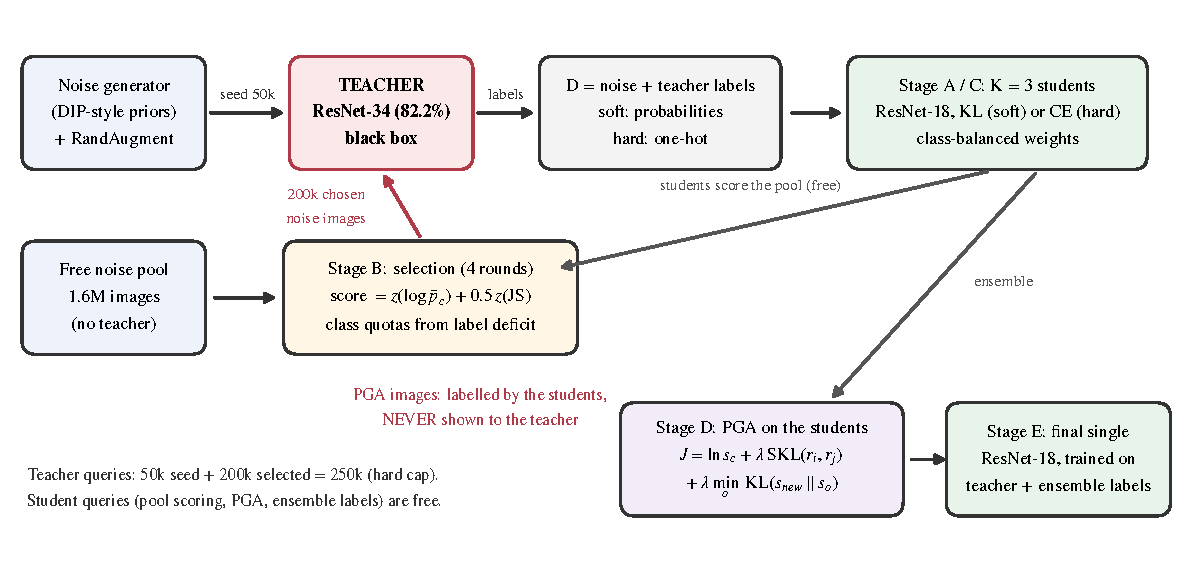
\includegraphics[width=1\textwidth,height=\textheight]{figs/fig1_pipeline.pdf}
\caption{Overview of the proposed pipeline (v2). Red arrows are the only
interactions with the teacher; all other computations use the students
and are free.}
\end{figure}

\begin{algorithm}[t]
\caption{Student-guided black-box distillation from noise (v2)}
\begin{algorithmic}[1]
\Require teacher oracle $T$, budget $B{=}250$K, seed size 50K, rounds $R{=}4$, students $K{=}3$
\Ensure student ResNet-18 $S_{\text{final}}$
\State $X_0\gets$ 50K noise images + RandAugment;\; $D\gets\{(x,T(x)) : x\in X_0\}$ \Comment{50K teacher queries}
\State Train students $S_{1..K}$ on $D$ (Eq.~\ref{eq:3}, weights Eq.~\ref{eq:4})
\For{$r=1,\dots,R$}
  \State Draw a pool $P$ of 400K free noise images; score all $(x,c)$ with Eq.~\ref{eq:8} \Comment{free}
  \State Compute class quotas from the label deficit (Eq.~\ref{eq:9}); take top-scoring images per class
  \State $D\gets D\cup\{(x,T(x))\}$ for the 50K chosen images \Comment{50K teacher queries}
  \State Fine-tune $S_{1..K}$ on $D$ for 10 epochs
\EndFor
\State Train fresh students $S_{1..K}$ on $D$ ($|D|=250$K) with class-balanced weights
\State $G_{\text{PGA}}\gets$ PGA on the ensemble (Eqs.~\ref{eq:5}--\ref{eq:7}); keep if all agree and conf.\ $\ge 0.8$ \Comment{never sent to $T$}
\State Label $G_{\text{PGA}}$ and 250K extra noise images with the ensemble \Comment{free}
\State $S_{\text{final}}\gets$ fine-tune the best student on $D\cup G$ (Eq.~\ref{eq:2})
\end{algorithmic}
\end{algorithm}

\hypertarget{noise-priors}{%
\subsection{Noise priors}\label{noise-priors}}

Following the supervisor's whiteboard design, the first seed sets
consisted of Gaussian, uniform, pink and Perlin noise. In a 10K-query
pilot with soft labels, a student trained on these reached only 5.1\%, a
mixture reached 8.6\%, and DIP-style priors {[}11{]} reached 11.5\%. All
reported experiments therefore use DIP-style priors. These are
hierarchical multi-scale noise with random rotations and elastic warps,
two of which (or one and a plain colour) are blended through a smooth
random blob mask, with per-image random colour and contrast. Every image
is further transformed by RandAugment {[}20{]} with two operations of
magnitude 9. Generation and augmentation run on the GPU. Representative
samples are shown in Fig. 2.

\hypertarget{distillation-with-class-balanced-weighting}{%
\subsection{Distillation with class-balanced
weighting}\label{distillation-with-class-balanced-weighting}}

Students are CIFAR-style ResNet-18 networks (3\$\times\$3 stem, no
max-pooling). They are trained with SGD and Nesterov momentum (0.9),
learning rate 0.1, weight decay \(5\cdot10^{-4}\), batch size 128, one
warm-up epoch followed by cosine decay, and random-crop and flip
augmentation.

The teacher's answers on noise are extremely imbalanced. On 250K random
noise images, the ten most frequent classes receive 52.6\% of all
labels, 39 classes receive fewer than 100 images, and 6 classes never
occur (Section 6.4). Each teacher-labelled image is therefore weighted
by

\begin{equation}w(x)=\operatorname{clip}\!\Big(\big(\bar n / n_{y(x)}\big)^{1/2},\;0.25,\;4\Big)\label{eq:4}\end{equation}

where \(n_y\) is the number of images labelled \(y\) and \(\bar n\) the
mean count. The weights are renormalised to mean one.

\begin{figure}
\centering
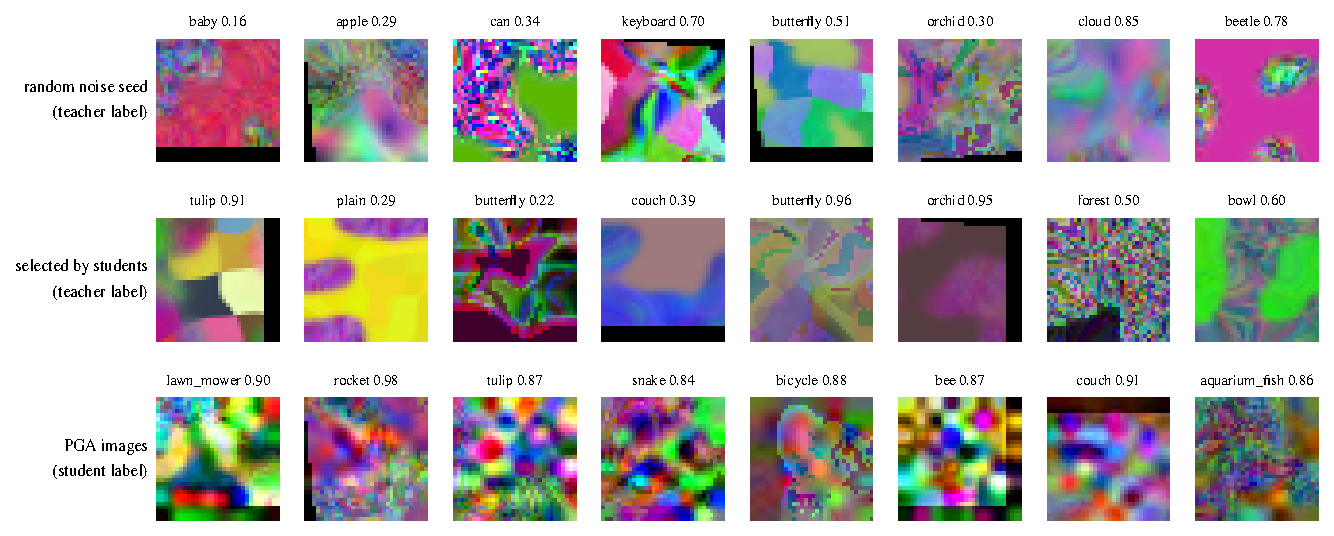
\includegraphics[width=1\textwidth,height=\textheight]{figs/fig2_examples.pdf}
\caption{Training images of the soft-label run. Top: random noise seed
with the teacher's label. Middle: noise images chosen by the students in
stage B, with the teacher's label. Bottom: PGA images with the students'
label; these are never shown to the teacher. Each title gives the label
and its probability.}
\end{figure}

\hypertarget{student-side-pga-with-softmax-space-diversity}{%
\subsection{Student-side PGA with softmax-space
diversity}\label{student-side-pga-with-softmax-space-diversity}}

Given target classes \(c_i\) for a batch of images, PGA \emph{maximises}
the following objective over the pixels while the student is frozen:

\begin{equation}\begin{aligned} J(x_i)&=\ln s_{c_i}(x_i)\;+\;\lambda_{\text{intra}}\,\frac{1}{|P_i|}\sum_{j\in P_i}\mathrm{SKL}\big(r(x_i),r(x_j)\big)\\ &\quad+\;\lambda_{\text{old}}\min_{o\in D,\;y_o=c_i}\mathrm{KL}\big(s(x_i)\,\|\,s(x_o)\big), \end{aligned}\label{eq:5}\end{equation}

where \(P_i\) is the set of other images in the batch with the same
target class, and

\begin{equation}r(x)_k=\frac{s_k(x)}{1-s_{c}(x)}\quad (k\neq c)\label{eq:6}\end{equation}

is the student's distribution over the 99 \emph{non-target} classes. The
three terms have distinct roles:

\begin{itemize}
\tightlist
\item
  \textbf{The first term} drives the image towards class \(c_i\).
\item
  \textbf{The second term} is the supervisor's diversity criterion: two
  images \(i\) and \(j\) of the same class must have different softmax
  outputs.
\item
  \textbf{The third term} pushes new images away from the closest
  existing data point of that class.
\end{itemize}

The diversity is measured on \(r\) rather than \(s\) deliberately. All
images of a class end with \(s_c\approx\tau_c\), so their full softmax
vectors are nearly identical. The non-target distribution, in contrast,
encodes \emph{what else an image resembles}: one ``orchid'' image may
lean towards ``tulip'' and another towards ``butterfly''. Each KL term
is capped at 5, so that diversity cannot override class attainment, and
\(\lambda_{\text{intra}}=\lambda_{\text{old}}=0.1\). The pixels are
updated by normalised momentum ascent with projection onto the valid
image range:

\begin{equation}g=\nabla_x J,\qquad m\leftarrow 0.9\,m+0.1\,g,\qquad x\leftarrow\Pi_{[0,1]}\Big(x+\alpha_t\,\frac{m}{\|m\|_2}\Big)\label{eq:7}\end{equation}

where:

\begin{itemize}
\tightlist
\item
  the step size \(\alpha_t\) decays from 0.5 to 0.1 over 300 steps
  (cosine schedule);
\item
  the gradient is restricted to a low-resolution subspace
  (8\$\times\(8, then 16\)\times\$16 once the confidence exceeds 0.5) to
  avoid high-frequency artefacts;
\item
  random shifts and flips are applied at every step;
\item
  an image stops once \(s_c\ge\tau_c\), with \(\tau_c\in\{0.8,0.9\}\);
\item
  images still below 0.3 confidence after 150 steps restart from fresh
  noise.
\end{itemize}

PGA is applied to the three-student ensemble with 200 targets per class
(20K in total). An image is retained only if \emph{all} students predict
its target class and the ensemble confidence is at least 0.8. Retained
images are labelled with the ensemble's probabilities and are never
shown to the teacher.

\hypertarget{student-guided-query-selection}{%
\subsection{Student-guided query
selection}\label{student-guided-query-selection}}

Spending the budget on random noise wastes most queries on a few
dominant classes. Instead, after a 50K random seed (stage A), the
remaining 200K queries are spent in four rounds of 50K. In each round
the students score a fresh pool of 400K free noise images. For image
\(x\) and class \(c\) the score is

\begin{equation}\text{score}_c(x)=z\big(\log\overline{p}_c(x)\big)+0.5\,z\big(\mathrm{JS}(x)\big),\qquad \mathrm{JS}(x)=\frac1K\sum_{k=1}^{K}\mathrm{KL}\big(p_k(x)\,\|\,\overline{p}(x)\big)\label{eq:8}\end{equation}

where JS is the generalised Jensen--Shannon disagreement of the \(K=3\)
students and \(z(\cdot)\) standardises a score over the pool, so that
both terms contribute on the same scale. Each class \(c\) receives a
quota

\begin{equation}q_c=n_r\Big(\frac{0.5}{100}+0.5\,\frac{\delta_c}{\sum_{c'}\delta_{c'}}\Big),\qquad \delta_c=\max\big(0,\;\bar n_{\text{target}}-n_c\big)\label{eq:9}\end{equation}

where \(n_r\) is the round size and \(\delta_c\) is the label deficit of
class \(c\) with respect to a perfectly balanced set. The classes with
the fewest labels select first, each taking its highest-scoring
unclaimed images. After each round the students are fine-tuned for 10
epochs, so that the next round is chosen by better students (active
learning).

\hypertarget{query-accounting}{%
\subsection{Query accounting}\label{query-accounting}}

Table 3 lists the cost of every stage. The oracle counts every query and
rejects any beyond the budget; for all main runs exactly 250,000 teacher
queries are issued, all on noise images.

\begin{longtable}[]{@{}
  >{\raggedright\arraybackslash}p{(\columnwidth - 6\tabcolsep) * \real{0.2222}}
  >{\centering\arraybackslash}p{(\columnwidth - 6\tabcolsep) * \real{0.2778}}
  >{\centering\arraybackslash}p{(\columnwidth - 6\tabcolsep) * \real{0.2778}}
  >{\raggedright\arraybackslash}p{(\columnwidth - 6\tabcolsep) * \real{0.2222}}@{}}
\caption{Teacher and student queries per stage (one v2 run). Student
passes are free under rule R4.}\tabularnewline
\toprule\noalign{}
\begin{minipage}[b]{\linewidth}\raggedright
Stage
\end{minipage} & \begin{minipage}[b]{\linewidth}\centering
Teacher queries
\end{minipage} & \begin{minipage}[b]{\linewidth}\centering
Student forward passes
\end{minipage} & \begin{minipage}[b]{\linewidth}\raggedright
Images involved
\end{minipage} \\
\midrule\noalign{}
\endfirsthead
\toprule\noalign{}
\begin{minipage}[b]{\linewidth}\raggedright
Stage
\end{minipage} & \begin{minipage}[b]{\linewidth}\centering
Teacher queries
\end{minipage} & \begin{minipage}[b]{\linewidth}\centering
Student forward passes
\end{minipage} & \begin{minipage}[b]{\linewidth}\raggedright
Images involved
\end{minipage} \\
\midrule\noalign{}
\endhead
\bottomrule\noalign{}
\endlastfoot
A --- random seed & 50,000 & --- & 50K noise images \\
B --- selection (4 rounds) & 200,000 & 4.8M & 1.6M pool \(\to\) 200K
chosen \\
C --- train students & 0 & --- & 250K teacher-labelled \\
D --- PGA & 0 & 6.0M & 20K targets \(\to\)
\$\approx\(11K kept | | E — consolidation | 0 | 0.75M | 250K extra noise | | **Total** | **250,000** | **\)\approx\$11.5M** \\
\end{longtable}

\hypertarget{experimental-setup}{%
\section{Experimental Setup}\label{experimental-setup}}

\textbf{Teacher.} The teacher is a CIFAR-style ResNet-34 trained for 200
epochs on 45,000 training images with SGD (learning rate 0.1, cosine
decay, weight decay \(5\cdot10^{-4}\)) and CutMix (probability 0.5). The
remaining 5,000 training images serve as a validation set. To avoid any
test-set selection bias, the checkpoint was chosen on validation (epoch
197: 82.50\% validation, 82.18\% test). After training, the teacher is
accessed exclusively through the query oracle.

\textbf{Configurations.} Table 4 lists the evaluated configurations. All
ablations of stages C--E reuse the teacher-labelled data of v2 (seed 1),
so they consume no additional queries and differ from v2 only in the
component under study.

\begin{longtable}[]{@{}
  >{\raggedright\arraybackslash}p{(\columnwidth - 2\tabcolsep) * \real{0.5000}}
  >{\raggedright\arraybackslash}p{(\columnwidth - 2\tabcolsep) * \real{0.5000}}@{}}
\caption{Evaluated configurations (each with soft and hard
labels).}\tabularnewline
\toprule\noalign{}
\begin{minipage}[b]{\linewidth}\raggedright
Name
\end{minipage} & \begin{minipage}[b]{\linewidth}\raggedright
Description
\end{minipage} \\
\midrule\noalign{}
\endfirsthead
\toprule\noalign{}
\begin{minipage}[b]{\linewidth}\raggedright
Name
\end{minipage} & \begin{minipage}[b]{\linewidth}\raggedright
Description
\end{minipage} \\
\midrule\noalign{}
\endhead
\bottomrule\noalign{}
\endlastfoot
Baseline & 1 student trained on 250K random noise images; no selection,
no PGA \\
Professor & Baseline + student-side PGA with diversity (Section 4.4) \\
v2 (ours) & Full pipeline of Section 4 (Algorithm 1) \\
v2 at 50K / 100K / 500K & Same pipeline at other budgets; the seed is
20\% of the budget \\
Baseline-500K & Baseline with a 500K budget \\
Ablations & Remove or modify one component of v2 (Table 7) \\
\end{longtable}

\textbf{Metrics and protocol.} We report top-1 accuracy on the 10,000
CIFAR-100 test images. Top-5 accuracy and teacher agreement are given in
Appendix D. The main configurations are run with three seeds (1, 2, 3)
and reported as mean \(\pm\) sample standard deviation; ablations use a
single seed.

\textbf{Compute.} All experiments ran on a single NVIDIA RTX 4000 Ada
GPU (20 GB). A v2 run takes about six hours when two runs share the GPU.
The complete study comprises 40 runs and about 75 hours of wall-clock
time on this GPU, with two or three runs sharing it.

\hypertarget{results}{%
\section{Results}\label{results}}

\hypertarget{main-results}{%
\subsection{Main results}\label{main-results}}

\begin{longtable}[]{@{}
  >{\raggedright\arraybackslash}p{(\columnwidth - 4\tabcolsep) * \real{0.2857}}
  >{\centering\arraybackslash}p{(\columnwidth - 4\tabcolsep) * \real{0.3571}}
  >{\centering\arraybackslash}p{(\columnwidth - 4\tabcolsep) * \real{0.3571}}@{}}
\caption{CIFAR-100 test accuracy (\%) with 250K teacher queries. Mean
\(\pm\) std over three seeds (baseline: two seeds; professor: one run).
Teacher: 82.18\%.}\tabularnewline
\toprule\noalign{}
\begin{minipage}[b]{\linewidth}\raggedright
Method
\end{minipage} & \begin{minipage}[b]{\linewidth}\centering
Soft labels
\end{minipage} & \begin{minipage}[b]{\linewidth}\centering
Hard labels
\end{minipage} \\
\midrule\noalign{}
\endfirsthead
\toprule\noalign{}
\begin{minipage}[b]{\linewidth}\raggedright
Method
\end{minipage} & \begin{minipage}[b]{\linewidth}\centering
Soft labels
\end{minipage} & \begin{minipage}[b]{\linewidth}\centering
Hard labels
\end{minipage} \\
\midrule\noalign{}
\endhead
\bottomrule\noalign{}
\endlastfoot
Baseline (random noise, 1 student) & 35.0 \(\pm\) 0.6 & 24.5 \(\pm\)
0.2 \\
Professor (+ student-side PGA with diversity) & 36.1 & 25.7 \\
\textbf{v2 --- final single student} & \textbf{41.4 \(\pm\) 0.6} &
\textbf{30.5 \(\pm\) 1.0} \\
\textbf{v2 --- ensemble of three students} & \textbf{43.0 \(\pm\) 0.2} &
\textbf{31.3 \(\pm\) 0.6} \\
Teacher (upper bound) & 82.2 & 82.2 \\
\end{longtable}

Table 5 summarises the main results. At the same budget, the proposed
pipeline improves the single student by \textbf{+6.4 points} with soft
labels and \textbf{+6.0 points} with hard labels. This is an order of
magnitude larger than the seed-to-seed standard deviation. The
supervisor's PGA refinement alone improves the baseline by +1.1 (soft)
and +1.2 (hard) points relative to the two-seed baseline mean. The
ensemble of three students is consistently 1--1.5 points more accurate
than the consolidated single student, and the top-5 accuracy of the
final soft-label student is 64.0\%.

\hypertarget{accuracy-as-a-function-of-the-query-budget}{%
\subsection{Accuracy as a function of the query
budget}\label{accuracy-as-a-function-of-the-query-budget}}

Fig. 3 and Table 6 support two conclusions:

\begin{enumerate}
\def\labelenumi{\arabic{enumi}.}
\tightlist
\item
  \textbf{Selecting which noise the teacher labels is worth more than
  doubling the budget.} With 250K queries v2 exceeds the 500K baseline:
  41.4 vs.~37.9 with soft labels and 30.5 vs.~27.3 with hard labels.
\item
  \textbf{The curve has not saturated.} Doubling the budget from 250K to
  500K still adds about three points, so the method remains limited by
  the amount of information obtained from the teacher.
\end{enumerate}

Hard labels are disproportionately affected at small budgets: with 50K
queries they reach only half the soft-label accuracy, since a class
index carries far less information than a probability vector.

\begin{figure}
\centering
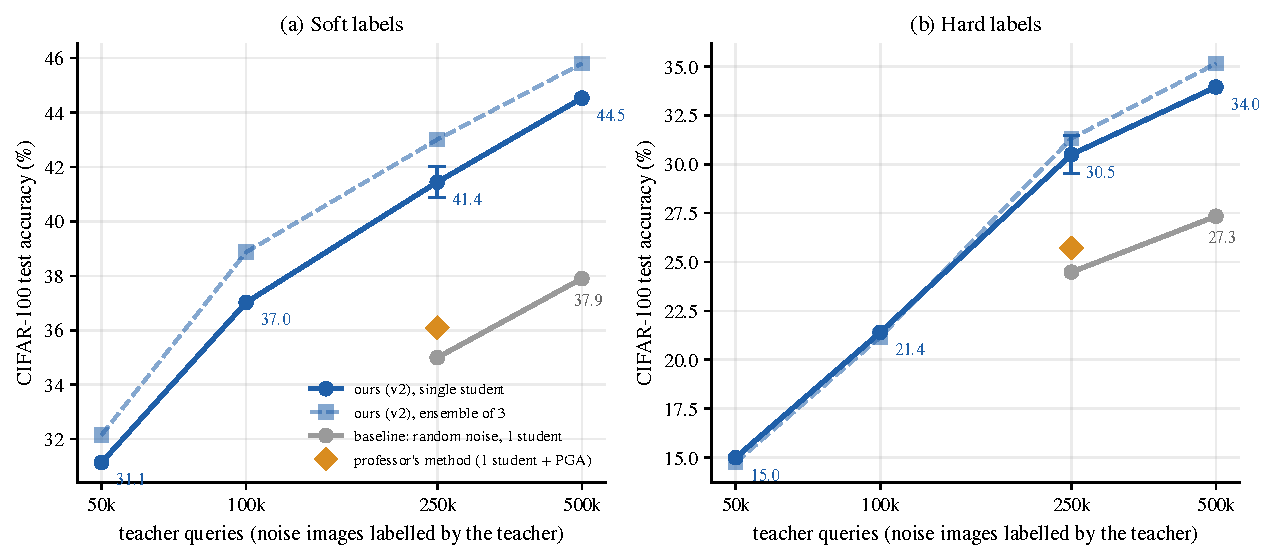
\includegraphics[width=0.9\textwidth,height=\textheight]{figs/fig3_budget.pdf}
\caption{Test accuracy against the number of teacher queries. The
proposed method with 250K queries outperforms the baseline with 500K
queries. The error bar shows \$\pm\$1 std over three seeds.}
\end{figure}

\begin{longtable}[]{@{}
  >{\raggedright\arraybackslash}p{(\columnwidth - 8\tabcolsep) * \real{0.1667}}
  >{\centering\arraybackslash}p{(\columnwidth - 8\tabcolsep) * \real{0.2083}}
  >{\centering\arraybackslash}p{(\columnwidth - 8\tabcolsep) * \real{0.2083}}
  >{\centering\arraybackslash}p{(\columnwidth - 8\tabcolsep) * \real{0.2083}}
  >{\centering\arraybackslash}p{(\columnwidth - 8\tabcolsep) * \real{0.2083}}@{}}
\caption{Budget sweep: final single student (ensemble in parentheses),
test accuracy in \%.}\tabularnewline
\toprule\noalign{}
\begin{minipage}[b]{\linewidth}\raggedright
Teacher queries
\end{minipage} & \begin{minipage}[b]{\linewidth}\centering
v2, soft
\end{minipage} & \begin{minipage}[b]{\linewidth}\centering
v2, hard
\end{minipage} & \begin{minipage}[b]{\linewidth}\centering
Baseline, soft
\end{minipage} & \begin{minipage}[b]{\linewidth}\centering
Baseline, hard
\end{minipage} \\
\midrule\noalign{}
\endfirsthead
\toprule\noalign{}
\begin{minipage}[b]{\linewidth}\raggedright
Teacher queries
\end{minipage} & \begin{minipage}[b]{\linewidth}\centering
v2, soft
\end{minipage} & \begin{minipage}[b]{\linewidth}\centering
v2, hard
\end{minipage} & \begin{minipage}[b]{\linewidth}\centering
Baseline, soft
\end{minipage} & \begin{minipage}[b]{\linewidth}\centering
Baseline, hard
\end{minipage} \\
\midrule\noalign{}
\endhead
\bottomrule\noalign{}
\endlastfoot
50K & 31.1 (32.2) & 15.0 (14.7) & --- & --- \\
100K & 37.0 (38.9) & 21.4 (21.2) & --- & --- \\
250K & 41.4 (43.0) & 30.5 (31.3) & 35.0 & 24.5 \\
500K & \textbf{44.5 (45.8)} & \textbf{34.0 (35.2)} & 37.9 & 27.3 \\
\end{longtable}

\hypertarget{ablation-study}{%
\subsection{Ablation study}\label{ablation-study}}

Fig. 4 and Table 7 isolate the contribution of each component.

\textbf{Selection is the decisive component.} Three students trained on
random noise without balancing are no better than a single student
(34.96\% vs.~35.0\%). Balanced selection with a single student already
yields +3.9 points, and three disagreeing students add another 1.5--3
points.

\textbf{PGA and diversity have no measurable effect on top of
selection.} Removing PGA, removing the diversity term, increasing it
tenfold, or generating five times as many PGA images changes accuracy by
at most 0.7 points, within about one seed standard deviation. In the
single-student setting, by contrast, PGA helps (Table 5). Section 6.5
analyses this discrepancy.

\textbf{CutMix is harmful (\$-\$5 points).} For natural images, CutMix
rests on the assumption that a mixture of two images has the
corresponding mixture of labels. On noise, the teacher's decision
depends on fine-grained texture statistics, and pasting a patch of one
image into another changes the prediction in ways that the interpolated
label does not describe.

\textbf{Two components of DIP-KD did not transfer.} Neither contrastive
pre-training on noise nor softening the hard labels with the ensemble
(DIP-KD's ``primer'' idea) improved our pipeline.

A final configuration (v3) combines every modification that improved on
v2 by more than 0.3 points. None qualified, so v3 reduces to a re-run of
v2 (40.8\% soft, 30.4\% hard), consistent with the seed variance.

\begin{figure}
\centering
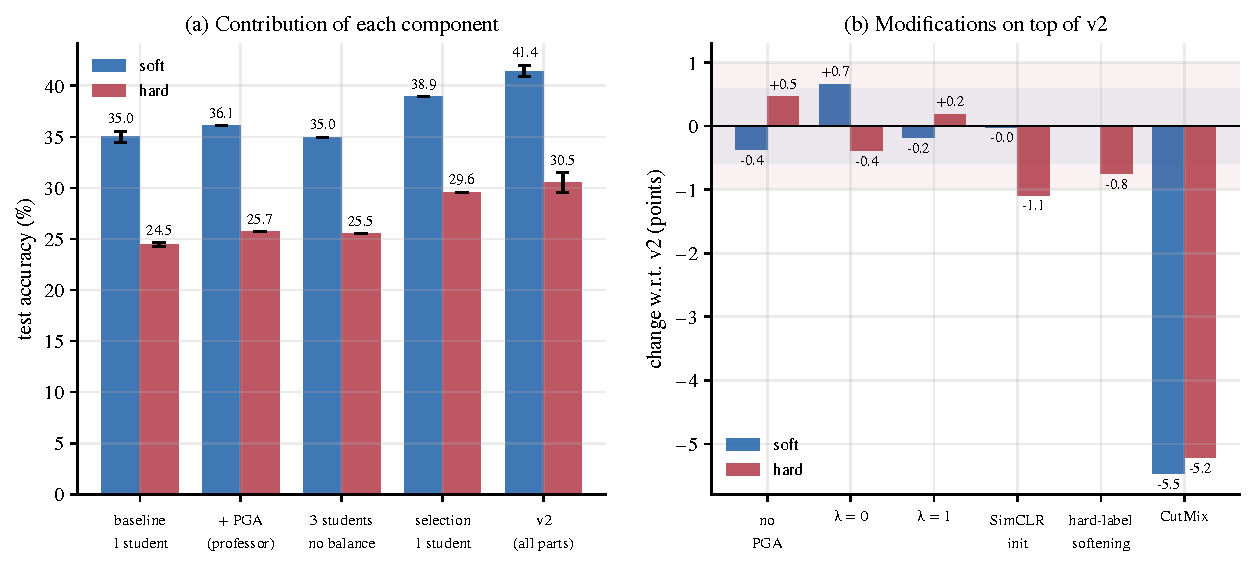
\includegraphics[width=0.92\textwidth,height=\textheight]{figs/fig6_ablations.pdf}
\caption{(a) Incremental contribution of the components at 250K queries.
(b) Change in accuracy relative to v2 (seed 1) when one component is
modified; the shaded band indicates \$\pm\$1 std across seeds.}
\end{figure}

\begin{longtable}[]{@{}
  >{\raggedright\arraybackslash}p{(\columnwidth - 8\tabcolsep) * \real{0.1667}}
  >{\centering\arraybackslash}p{(\columnwidth - 8\tabcolsep) * \real{0.2083}}
  >{\centering\arraybackslash}p{(\columnwidth - 8\tabcolsep) * \real{0.2083}}
  >{\centering\arraybackslash}p{(\columnwidth - 8\tabcolsep) * \real{0.2083}}
  >{\centering\arraybackslash}p{(\columnwidth - 8\tabcolsep) * \real{0.2083}}@{}}
\caption{Ablations at 250K queries (final single student, \%).
\(\Delta\) is relative to v2 seed 1 (42.03 soft / 31.04
hard).}\tabularnewline
\toprule\noalign{}
\begin{minipage}[b]{\linewidth}\raggedright
Variant
\end{minipage} & \begin{minipage}[b]{\linewidth}\centering
Soft
\end{minipage} & \begin{minipage}[b]{\linewidth}\centering
\(\Delta\)
\end{minipage} & \begin{minipage}[b]{\linewidth}\centering
Hard
\end{minipage} & \begin{minipage}[b]{\linewidth}\centering
\(\Delta\)
\end{minipage} \\
\midrule\noalign{}
\endfirsthead
\toprule\noalign{}
\begin{minipage}[b]{\linewidth}\raggedright
Variant
\end{minipage} & \begin{minipage}[b]{\linewidth}\centering
Soft
\end{minipage} & \begin{minipage}[b]{\linewidth}\centering
\(\Delta\)
\end{minipage} & \begin{minipage}[b]{\linewidth}\centering
Hard
\end{minipage} & \begin{minipage}[b]{\linewidth}\centering
\(\Delta\)
\end{minipage} \\
\midrule\noalign{}
\endhead
\bottomrule\noalign{}
\endlastfoot
3 students, random 250K, no balancing & 34.96 & \$-\$7.1 & 25.55 &
\$-\$5.5 \\
Balanced selection, 1 student & 38.93 & \$-\$3.1 & 29.58 & \$-\$1.5 \\
v2 without PGA & 41.66 & \$-\$0.4 & 31.50 & +0.5 \\
v2, PGA with \(\lambda\) = 0 (no diversity) & 42.69 & +0.7 & 30.65 &
\$-\$0.4 \\
v2, PGA with \(\lambda\) = 1.0 (10\(\times\) diversity) & 41.85 &
\$-\(0.2 | 31.23 | +0.2 | | v2, 5\)\times\$ more PGA images (100K) &
42.63 & +0.6 \\
v2 + contrastive (SimCLR) pre-training on noise & 42.01 & 0.0 & 29.95 &
\$-\$1.1 \\
v2 + hard labels softened by the ensemble & --- & --- & 30.29 &
\$-\(0.8 | | v2 + CutMix | 36.56 | **\)-\(5.5** | 25.82 | **\)-\$5.2** \\
\end{longtable}

\hypertarget{why-selection-works}{%
\subsection{Why selection works}\label{why-selection-works}}

\textbf{The teacher maps most noise to a few classes.} Fig. 5 reveals
the central difficulty of noise-only distillation, and selection
mitigates it substantially (Table 8). The entropy of the teacher's label
distribution bounds the information that a hard label can convey about
the class. It rises from 5.11 to 5.54 bits per query (the maximum is
\(\log_2 100=6.64\)), which corresponds to an increase in the effective
number of covered classes from 34.6 to 46.7.

\begin{longtable}[]{@{}lcc@{}}
\caption{Statistics of the teacher-labelled set (250K queries,
soft-label runs).}\tabularnewline
\toprule\noalign{}
& Random noise & Student-selected \\
\midrule\noalign{}
\endfirsthead
\toprule\noalign{}
& Random noise & Student-selected \\
\midrule\noalign{}
\endhead
\bottomrule\noalign{}
\endlastfoot
Share of the ten most frequent classes & 52.6\% & 42.0\% \\
Classes with fewer than 100 images & 39 & 31 \\
Classes never labelled & 6 & 5 \\
Entropy of the label distribution & 5.11 bits & 5.54 bits \\
Effective number of classes (\(2^{H}\)) & 34.6 & 46.7 \\
Classes with 0\% test accuracy & 32 & 22 \\
\end{longtable}

\begin{figure}
\centering
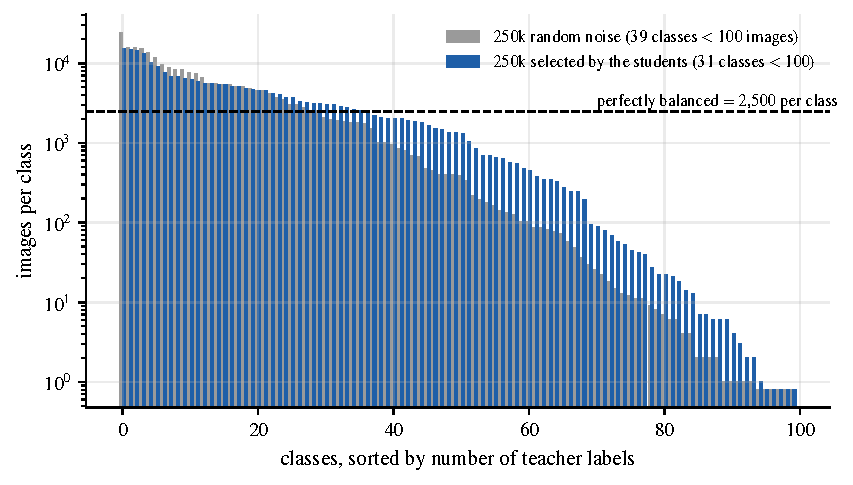
\includegraphics[width=0.74\textwidth,height=\textheight]{figs/fig4_imbalance.pdf}
\caption{Number of teacher labels per class (log scale) for 250K random
noise images and for the 250K images selected by the students.}
\end{figure}

\textbf{Per-class accuracy is governed by label coverage.} Fig. 6(a)
shows that a class is learned only if the teacher labelled enough noise
images with it: the Spearman correlation between label count and
accuracy is 0.81 for the baseline. Selection reduces the number of
classes with 0\% test accuracy from 32 to 22, and the number below 10\%
from 39 to 26. Overall, 45 classes improve and 29 degrade (Fig. 6(b)).
The strongest gains, of up to 80 points, occur for classes that the
baseline almost never saw.

\begin{figure}
\centering
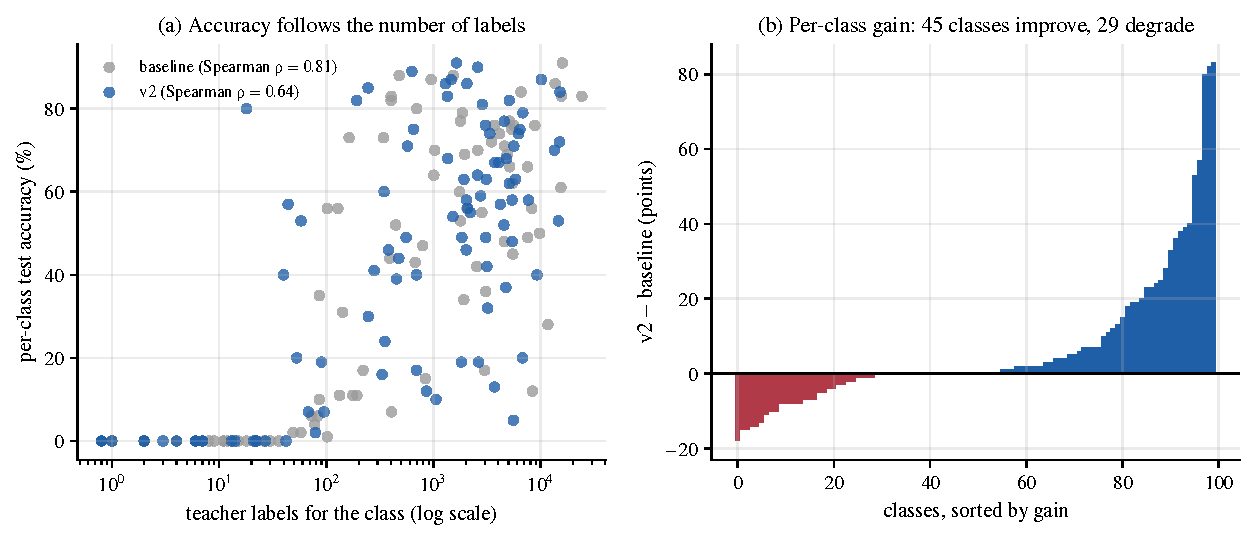
\includegraphics[width=0.92\textwidth,height=\textheight]{figs/fig8_perclass.pdf}
\caption{(a) Per-class test accuracy against the number of teacher
labels of that class, for the baseline and for v2 (soft labels). (b)
Per-class change in accuracy from the baseline to v2.}
\end{figure}

\textbf{Each round produces better selectors.} The soft-label ensemble
improves after every round: 25.7 \(\to\) 32.3 \(\to\) 37.1 \(\to\)
38.8\% after rounds 1--3, and 43.2\% after the stage-C retraining (Fig.
7(a)). The teacher returns the class targeted by the students for about
19--21\% of the selected images with soft labels and 9--11\% with hard
labels, against 1\% by chance (Fig. 7(b)). The selected images have
about twice the student disagreement of the pool (0.135 vs.~0.066 in
round 1). The budget is thus spent on rare classes and on images where
the students are uncertain, which are exactly the queries whose answers
are most informative. This is the principle of DisGUIDE {[}7{]} and
CaBaGE {[}10{]}, applied here to \emph{choosing among noise} rather than
to \emph{training a generator against the teacher}.

\begin{figure}
\centering
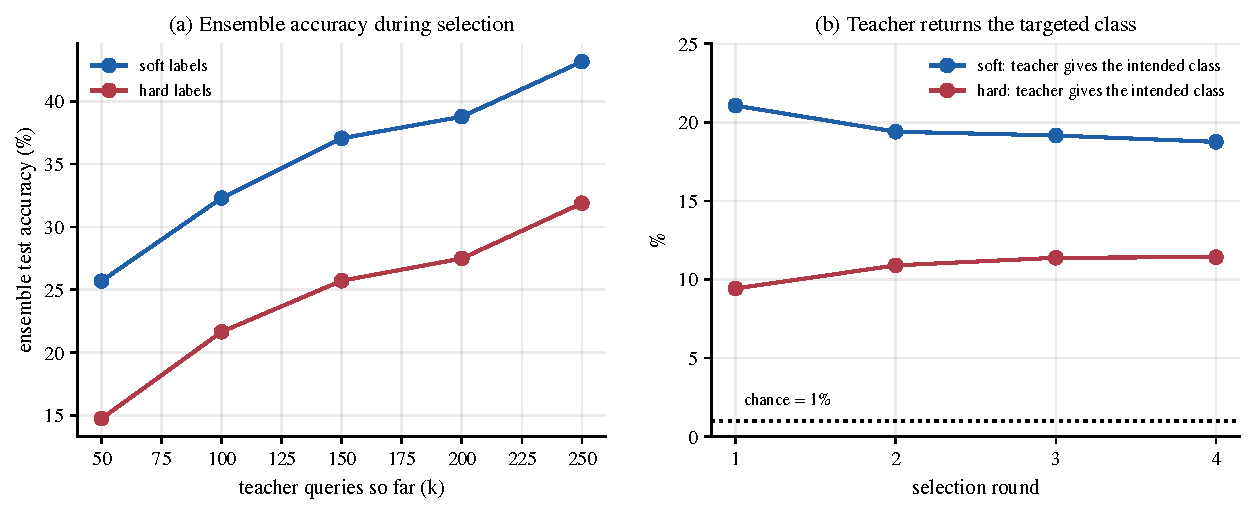
\includegraphics[width=0.86\textwidth,height=\textheight]{figs/fig5_rounds.pdf}
\caption{(a) Ensemble accuracy after each selection round. (b) Fraction
of selected images for which the teacher returns the class the students
targeted (chance: 1\%).}
\end{figure}

\hypertarget{effect-of-the-diversity-term}{%
\subsection{Effect of the diversity
term}\label{effect-of-the-diversity-term}}

Each PGA image may be viewed as a \emph{point} in the student's
probability space. The intra-class term of Eq. 5 increases
\(\mathrm{SKL}(r_i,r_j)\) and thereby pushes points of the same class
apart. The second term pushes each point away from its nearest existing
neighbour of the same class.

\textbf{The mechanism works as intended.} The mean pairwise symmetric KL
between same-class images grows almost fivefold, from 0.75 to 3.47
(Table 9). Without diversity, the samples of a class form a single tight
cluster. With \(\lambda\) = 1 they spread along several directions, each
pointing towards a different neighbouring class (Fig. 8).

\textbf{Diversity comes at a cost.} Strongly diversified images reach
the target confidence far less often (13.5\% vs.~46\%), so only a third
as many are retained.

\textbf{It does not improve accuracy.} The PGA images carry no new
information about the teacher, because they are labelled by the students
themselves. Making them more diverse cannot correct the students' own
errors, so they act only as a regulariser. This regularisation is useful
for a weak single student trained on random noise (+1.1 to +1.2 points),
but is redundant for an ensemble that was already trained on
well-selected teacher labels.

\textbf{Label reliability of PGA images.} For analysis only, after all
experiments we evaluated the teacher on the retained PGA images; these
answers never influenced training or selection. The teacher agrees with
the students' labels for 90.5\% of the soft-label images but only 56.2\%
of the hard-label images. Students trained on one-hot targets are
over-confident on synthetic inputs, which makes the
agreement-and-confidence filter less reliable in the hard-label setting.

\begin{figure}
\centering
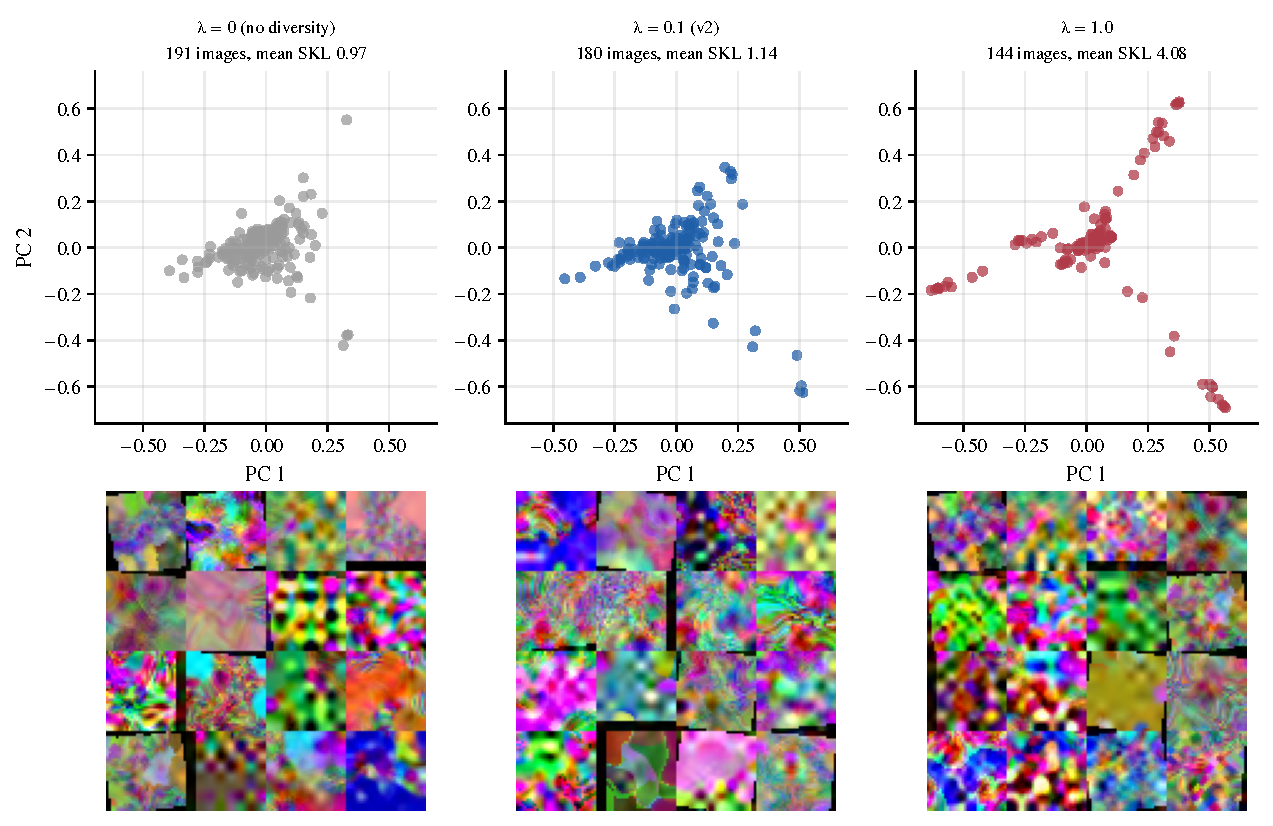
\includegraphics[width=0.8\textwidth,height=\textheight]{figs/fig7_diversity.pdf}
\caption{PGA images of the class ``orchid'' for \(\lambda\) = 0, 0.1 and
1.0 (left to right). Top: each point is one image, placed by its
non-target student distribution r(x), projected onto the first two
principal components. Bottom: sixteen example images. Increasing
\(\lambda\) spreads same-class images apart in the student's softmax
space.}
\end{figure}

\begin{longtable}[]{@{}
  >{\raggedright\arraybackslash}p{(\columnwidth - 6\tabcolsep) * \real{0.2105}}
  >{\centering\arraybackslash}p{(\columnwidth - 6\tabcolsep) * \real{0.2632}}
  >{\centering\arraybackslash}p{(\columnwidth - 6\tabcolsep) * \real{0.2632}}
  >{\centering\arraybackslash}p{(\columnwidth - 6\tabcolsep) * \real{0.2632}}@{}}
\caption{Effect of the diversity weight \(\lambda\) (soft labels; PGA
statistics over all classes).}\tabularnewline
\toprule\noalign{}
\begin{minipage}[b]{\linewidth}\raggedright
\end{minipage} & \begin{minipage}[b]{\linewidth}\centering
\(\lambda\) = 0
\end{minipage} & \begin{minipage}[b]{\linewidth}\centering
\(\lambda\) = 0.1 (v2)
\end{minipage} & \begin{minipage}[b]{\linewidth}\centering
\(\lambda\) = 1.0
\end{minipage} \\
\midrule\noalign{}
\endfirsthead
\toprule\noalign{}
\begin{minipage}[b]{\linewidth}\raggedright
\end{minipage} & \begin{minipage}[b]{\linewidth}\centering
\(\lambda\) = 0
\end{minipage} & \begin{minipage}[b]{\linewidth}\centering
\(\lambda\) = 0.1 (v2)
\end{minipage} & \begin{minipage}[b]{\linewidth}\centering
\(\lambda\) = 1.0
\end{minipage} \\
\midrule\noalign{}
\endhead
\bottomrule\noalign{}
\endlastfoot
Mean pairwise SKL between same-class images & 0.75 & 1.15 &
\textbf{3.47} \\
PGA images retained (of 20K) & 10,906 & 10,778 & 3,289 \\
Images reaching the target confidence & 47.5\% & 46.2\% & 13.5\% \\
Teacher agrees with retained labels (diagnostic) & 91.4\% & 90.5\% &
86.9\% \\
Final student accuracy & 42.69 & 42.03 & 41.85 \\
\end{longtable}

\hypertarget{comparison-with-prior-work}{%
\subsection{Comparison with prior
work}\label{comparison-with-prior-work}}

\begin{longtable}[]{@{}
  >{\raggedright\arraybackslash}p{(\columnwidth - 10\tabcolsep) * \real{0.1379}}
  >{\centering\arraybackslash}p{(\columnwidth - 10\tabcolsep) * \real{0.1724}}
  >{\centering\arraybackslash}p{(\columnwidth - 10\tabcolsep) * \real{0.1724}}
  >{\centering\arraybackslash}p{(\columnwidth - 10\tabcolsep) * \real{0.1724}}
  >{\centering\arraybackslash}p{(\columnwidth - 10\tabcolsep) * \real{0.1724}}
  >{\centering\arraybackslash}p{(\columnwidth - 10\tabcolsep) * \real{0.1724}}@{}}
\caption{Comparison with published CIFAR-100 results at their reported
query budgets. ``\(\approx\)'' marks approximate values or values from a
secondary source; the teachers differ between rows.}\tabularnewline
\toprule\noalign{}
\begin{minipage}[b]{\linewidth}\raggedright
Method
\end{minipage} & \begin{minipage}[b]{\linewidth}\centering
Labels
\end{minipage} & \begin{minipage}[b]{\linewidth}\centering
Teacher queries
\end{minipage} & \begin{minipage}[b]{\linewidth}\centering
Teacher
\end{minipage} & \begin{minipage}[b]{\linewidth}\centering
Student
\end{minipage} & \begin{minipage}[b]{\linewidth}\centering
Student / teacher
\end{minipage} \\
\midrule\noalign{}
\endfirsthead
\toprule\noalign{}
\begin{minipage}[b]{\linewidth}\raggedright
Method
\end{minipage} & \begin{minipage}[b]{\linewidth}\centering
Labels
\end{minipage} & \begin{minipage}[b]{\linewidth}\centering
Teacher queries
\end{minipage} & \begin{minipage}[b]{\linewidth}\centering
Teacher
\end{minipage} & \begin{minipage}[b]{\linewidth}\centering
Student
\end{minipage} & \begin{minipage}[b]{\linewidth}\centering
Student / teacher
\end{minipage} \\
\midrule\noalign{}
\endhead
\bottomrule\noalign{}
\endlastfoot
ZSDB3KD {[}2{]} (as reported in {[}6{]}) & hard & 2M & 89.45\% & 17.51\%
& 0.20 \\
DFME {[}3{]} (as reported in {[}6{]}) & hard & 2M & 89.45\% & 20.01\% &
0.22 \\
IDEAL {[}6{]} & hard & 2M & 89.45\% & 36.96\% & 0.41 \\
DisGUIDE {[}7{]} & hard & \$\approx\$10M & --- & \$\approx\$50\% &
--- \\
DFHL-RS {[}9{]} (robust teacher) & hard & \$\approx\$77M & 56.76\% &
51.94\% & 0.92 \\
CaBaGE {[}10{]} & soft & millions & 77.52\% & 75.96\% & 0.98 \\
Diffusion attack {[}12{]} & hard & 150K & --- & \$\approx\$57--60\% &
--- \\
IDEAL (as reported in {[}11{]}) & hard & 100K & 78.36\% & 33.64\% &
0.43 \\
DFHL-RS (as reported in {[}11{]}) & hard & 100K & 78.36\% & 51.97\% &
0.66 \\
DIP-KD {[}11{]} & hard & 100K & 78.36\% & 52.85\% & 0.67 \\
\textbf{Ours (v2)} & \textbf{hard} & \textbf{100K} & \textbf{82.18\%} &
\textbf{21.4\%} & \textbf{0.26} \\
\textbf{Ours (v2)} & \textbf{hard} & \textbf{250K} & \textbf{82.18\%} &
\textbf{30.5\%} & \textbf{0.37} \\
\textbf{Ours (v2)} & \textbf{hard} & \textbf{500K} & \textbf{82.18\%} &
\textbf{34.0\%} & \textbf{0.41} \\
\textbf{Ours (v2)} & \textbf{soft} & \textbf{250K} & \textbf{82.18\%} &
\textbf{41.4\%} & \textbf{0.50} \\
\end{longtable}

Table 10 places our results in context.

\textbf{Query efficiency against generator-based methods.} Relative to
methods that train generators with millions of queries, our approach is
query-efficient. With 4\(\times\) fewer queries than IDEAL (500K
vs.~2M), it recovers the same fraction of the teacher's accuracy (0.41).
With 8\(\times\) fewer queries it clearly exceeds ZSDB3KD and DFME
evaluated at 2M. This is despite a stricter protocol: every
generator-based method sends the teacher images optimised for the
attack, whereas our teacher only sees random noise. Because our queries
are plain noise, they reveal nothing about which classes the attacker is
interested in, although noise itself is easily flagged by an
out-of-distribution detector.

\textbf{The gap to fixed-prior methods.} At an equal budget of 100K
hard-label queries, DIP-KD reports 52.85\% against our 21.4\%. Two of
DIP-KD's three components (contrastive learning and soft-label priming)
did not help in our pipeline (Table 7). This suggests that its advantage
stems mainly from its image priors, semantic CutMix of structured
patterns, which raise the information content of each query. The
teachers and protocols also differ: DIP-KD's teacher is weaker
(78.36\%), and its synthetic set may be augmented differently.

\textbf{Soft-label methods.} With soft labels, CaBaGE recovers 98\% of
its teacher, but it uses millions of queries and generators trained
against the teacher.

\hypertarget{discussion}{%
\section{Discussion}\label{discussion}}

\textbf{Why noise-only distillation plateaus.} Our results consistently
indicate that the bottleneck lies on the teacher side. Every
intervention that increases the information obtained from the teacher
(class-balanced selection, student disagreement, a larger budget)
improves accuracy. Every intervention that only reshapes student-side
data (PGA diversity, more PGA images, CutMix, contrastive pre-training)
does not. Two effects drive this:

\begin{itemize}
\tightlist
\item
  The teacher assigns random noise to a small number of classes
  (effective number 34.6 of 100).
\item
  A class is only learned if it receives enough labels: per-class
  accuracy correlates with label count at \(\rho\) = 0.81.
\end{itemize}

Consequently, roughly a fifth of the classes remain unlearned even after
selection.

\textbf{Limitations.}

\begin{itemize}
\tightlist
\item
  \emph{Absolute accuracy.} It remains far below the teacher: about 50\%
  (soft) and 37\% (hard) of the teacher's accuracy at 250K queries. No
  published method approaches the teacher from pure noise at this
  budget.
\item
  \emph{Statistical power.} Most ablations use a single seed, and their
  effects, apart from selection and CutMix, are within one seed standard
  deviation. They should be read as ``no measurable effect'' rather than
  as evidence of harm or benefit.
\item
  \emph{Diagnostic evaluation.} The label-quality analysis evaluated the
  teacher on PGA images after training. It never influenced any model,
  but it would be unavailable in a real deployment.
\item
  \emph{Final consolidation.} Stage E does not improve on the best
  stage-C student; the ensemble remains the most accurate model.
\end{itemize}

\textbf{An instructive exception.} In an exploratory run that violated
rule R3 and is excluded from all reported results, sending PGA images to
the teacher reached 36.8\% with soft labels and only 150K queries.
Teacher-labelled, class-targeted images are therefore highly
informative, which explains why most of the literature optimises the
teacher's queries directly.

\textbf{Broader impact.} Black-box distillation is dual-use: the same
techniques that compress models can be used to copy proprietary ones. By
quantifying how many noise queries are needed to recover a given
fraction of a teacher's accuracy, this study informs the design of query
limits. It also suggests that simple out-of-distribution detection of
noise-like queries would be an effective defence against attacks of the
kind studied here.

\hypertarget{conclusion}{%
\section{Conclusion}\label{conclusion}}

We implemented the supervisor's black-box, noise-only distillation
method with student-side PGA and softmax-space diversity, and extended
it with student-guided, class-balanced query selection over a pool of
free noise.

\begin{itemize}
\tightlist
\item
  With 250K teacher queries, the method improves the student by about
  six points (41.4\% soft, 30.5\% hard over three seeds), and it
  outperforms a baseline given twice the budget.
\item
  The diversity term demonstrably spreads same-class synthetic images
  apart in the student's softmax space. However, these images carry no
  teacher information, so the term does not raise accuracy once the
  teacher's queries are chosen well.
\end{itemize}

We see three directions for future work, in order of expected impact:

\begin{enumerate}
\def\labelenumi{\arabic{enumi}.}
\tightlist
\item
  Richer procedural image priors, such as dead-leaves models, fractals,
  randomly initialised generators and semantic CutMix, to increase the
  information content of each query.
\item
  Steering pool images towards under-represented classes with the
  students \emph{before} querying, which requires relaxing rule R3.
\item
  Larger free pools and more selection rounds.
\end{enumerate}

\hypertarget{references}{%
\section*{References}\label{references}}
\addcontentsline{toc}{section}{References}

\begin{enumerate}
\def\labelenumi{\arabic{enumi}.}
\tightlist
\item
  G. Hinton, O. Vinyals, and J. Dean. Distilling the knowledge in a
  neural network. \emph{NeurIPS Deep Learning Workshop}, 2015.
\item
  Z. Wang. Zero-shot knowledge distillation from a decision-based
  black-box model. In \emph{ICML}, 2021.
\item
  J.-B. Truong, P. Maini, R. J. Walls, and N. Papernot. Data-free model
  extraction. In \emph{CVPR}, 2021.
\item
  S. Kariyappa, A. Prakash, and M. K. Qureshi. MAZE: Data-free model
  stealing attack using zeroth-order gradient estimation. In
  \emph{CVPR}, 2021.
\item
  S. Sanyal, S. Addepalli, and R. V. Babu. Towards data-free model
  stealing in a hard label setting. In \emph{CVPR}, 2022.
\item
  J. Zhang, C. Chen, and L. Lyu. IDEAL: Query-efficient data-free
  learning from black-box models. In \emph{ICLR}, 2023.
\item
  J. Rosenthal, E. Enouen, H. V. Pham, and L. Tan. DisGUIDE:
  Disagreement-guided data-free model extraction. In \emph{AAAI}, 2023.
\item
  J. Beetham, N. Kardan, A. Mian, and M. Shah. Dual student networks for
  data-free model stealing. In \emph{ICLR}, 2023.
\item
  X. Yuan, K. Chen, W. Huang, J. Zhang, W. Zhang, and N. Yu. Data-free
  hard-label robustness stealing attack. In \emph{AAAI}, 2024.
\item
  J. Rosenthal, S. Liang, K. Zhang, and L. Tan. CaBaGE: Data-free model
  extraction using class balanced generator ensemble.
  \emph{arXiv:2409.10643}, 2024.
\item
  Diverse image priors for black-box data-free knowledge distillation
  (DIP-KD). \emph{arXiv:2604.25794}, 2026.
\item
  Explore the vulnerability of black-box models via diffusion models.
  \emph{arXiv:2506.07590}, 2025.
\item
  S. Pal, Y. Gupta, A. Shukla, A. Kanade, S. Shevade, and V. Ganapathy.
  ActiveThief: Model extraction using active learning and unannotated
  public data. In \emph{AAAI}, 2020.
\item
  Class imbalance in active-learning-based model extraction. In
  \emph{IJCAI}, 2024.
\item
  M. Baradad, J. Wulff, T. Wang, P. Isola, and A. Torralba. Learning to
  see by looking at noise. In \emph{NeurIPS}, 2021.
\item
  H. Yin, P. Molchanov, J. M. Alvarez, Z. Li, A. Mallya, D. Hoiem, N. K.
  Jha, and J. Kautz. Dreaming to distill: Data-free knowledge transfer
  via DeepInversion. In \emph{CVPR}, 2020.
\item
  Mukherjee et al.~ZOPGA-KD. \emph{arXiv:2611.00908}, 2026.
\item
  T. Chen, S. Kornblith, M. Norouzi, and G. Hinton. A simple framework
  for contrastive learning of visual representations. In \emph{ICML},
  2020.
\item
  S. Yun, D. Han, S. J. Oh, S. Chun, J. Choe, and Y. Yoo. CutMix:
  Regularization strategy to train strong classifiers with localizable
  features. In \emph{ICCV}, 2019.
\item
  E. D. Cubuk, B. Zoph, J. Shlens, and Q. V. Le. RandAugment: Practical
  automated data augmentation with a reduced search space. In \emph{CVPR
  Workshops}, 2020.
\item
  H. Chen, Y. Wang, C. Xu, Z. Yang, C. Liu, B. Shi, C. Xu, C. Xu, and Q.
  Tian. Data-free learning of student networks. In \emph{ICCV}, 2019.
\item
  G. Fang, J. Song, X. Wang, C. Shen, X. Wang, and M. Song. Contrastive
  model inversion for data-free knowledge distillation. In \emph{IJCAI},
  2021.
\item
  T. Orekondy, B. Schiele, and M. Fritz. Knockoff nets: Stealing
  functionality of black-box models. In \emph{CVPR}, 2019.
\item
  MGCT: Multi-generator collaborative training for data-free model
  stealing. \emph{Cybersecurity}, Springer, 2025.
\item
  Stabilizing data-free model extraction. \emph{arXiv:2509.11159}, 2025.
\end{enumerate}

\hypertarget{appendix-a-hyperparameters}{%
\section*{Appendix A:
Hyperparameters}\label{appendix-a-hyperparameters}}
\addcontentsline{toc}{section}{Appendix A: Hyperparameters}

\begin{longtable}[]{@{}
  >{\raggedright\arraybackslash}p{(\columnwidth - 2\tabcolsep) * \real{0.5000}}
  >{\raggedright\arraybackslash}p{(\columnwidth - 2\tabcolsep) * \real{0.5000}}@{}}
\caption{Hyperparameters of the v2 pipeline.}\tabularnewline
\toprule\noalign{}
\begin{minipage}[b]{\linewidth}\raggedright
Component
\end{minipage} & \begin{minipage}[b]{\linewidth}\raggedright
Setting
\end{minipage} \\
\midrule\noalign{}
\endfirsthead
\toprule\noalign{}
\begin{minipage}[b]{\linewidth}\raggedright
Component
\end{minipage} & \begin{minipage}[b]{\linewidth}\raggedright
Setting
\end{minipage} \\
\midrule\noalign{}
\endhead
\bottomrule\noalign{}
\endlastfoot
Noise & DIP-style priors + RandAugment (2 operations, magnitude 9),
generated on the GPU \\
Student & ResNet-18 (CIFAR stem), SGD + Nesterov 0.9, lr 0.1, weight
decay 5e-4, batch 128, cosine schedule, crop + flip \\
Distillation loss & soft: KL divergence at temperature \(\tau=4\)
(scaled by \(\tau^2\)); hard: cross-entropy \\
Class weights & \((\bar n/n_y)^{1/2}\), clipped to \([0.25, 4]\),
renormalised to mean 1 (Eq. 4) \\
Stage A & 50K seed, 3 students, 60 epochs \\
Stage B & 4 rounds \(\times\) 50K; 400K pool per round; score Eq. 8 with
disagreement weight 0.5; quotas Eq. 9; 10 fine-tuning epochs at lr 0.05
between rounds \\
Stage C & 3 fresh students, 40 epochs on 250K images \\
Stage D (PGA) & 20K targets (200 per class); 300 steps; step 0.5 \(\to\)
0.1 (cosine); momentum 0.9; \(\tau_c\in\{0.8,0.9\}\);
\(\lambda_{\text{intra}}=\lambda_{\text{old}}=0.1\); KL cap 5;
low-resolution gradient 8\$\times\(8 / 16\)\times\$16; restart below 0.3
at step 150; keep if all students agree and confidence \(\ge\) 0.8 \\
Stage E & initialise from the best stage-C student; 10 epochs at lr
0.02; teacher-labelled data + PGA + 250K extra noise (ensemble labels,
weight 0.5) \\
Seeds & 1, 2, 3 \\
\end{longtable}

\hypertarget{appendix-b-development-history}{%
\section*{Appendix B: Development
History}\label{appendix-b-development-history}}
\addcontentsline{toc}{section}{Appendix B: Development History}

\begin{longtable}[]{@{}
  >{\raggedright\arraybackslash}p{(\columnwidth - 6\tabcolsep) * \real{0.2105}}
  >{\centering\arraybackslash}p{(\columnwidth - 6\tabcolsep) * \real{0.2632}}
  >{\centering\arraybackslash}p{(\columnwidth - 6\tabcolsep) * \real{0.2632}}
  >{\centering\arraybackslash}p{(\columnwidth - 6\tabcolsep) * \real{0.2632}}@{}}
\caption{Development of the method (earlier teacher with 82.37\%
accuracy, checkpoint chosen on the test set).}\tabularnewline
\toprule\noalign{}
\begin{minipage}[b]{\linewidth}\raggedright
Stage of the project
\end{minipage} & \begin{minipage}[b]{\linewidth}\centering
Teacher queries
\end{minipage} & \begin{minipage}[b]{\linewidth}\centering
Soft
\end{minipage} & \begin{minipage}[b]{\linewidth}\centering
Hard
\end{minipage} \\
\midrule\noalign{}
\endfirsthead
\toprule\noalign{}
\begin{minipage}[b]{\linewidth}\raggedright
Stage of the project
\end{minipage} & \begin{minipage}[b]{\linewidth}\centering
Teacher queries
\end{minipage} & \begin{minipage}[b]{\linewidth}\centering
Soft
\end{minipage} & \begin{minipage}[b]{\linewidth}\centering
Hard
\end{minipage} \\
\midrule\noalign{}
\endhead
\bottomrule\noalign{}
\endlastfoot
Whiteboard noise (Gaussian / uniform / pink / Perlin), 10K seed & 10K &
5.1 & --- \\
DIP-style noise, 10K seed & 10K & 11.5 & --- \\
DIP noise, 50K seed + unfiltered student-labelled PGA & 50K & 25.8
\(\to\) 23.4 & 11.9 \(\to\) 9.5 \\
DIP noise, 250K seed + filtered student-labelled PGA & 250K & 34.6
\(\to\) 34.1 & 23.5 \(\to\) 23.3 \\
v1: 3 students, one-shot class-balanced selection & 250K & 36.2 (ens.
37.8) & 27.4 (ens. 28.7) \\
\textbf{v2: final method, retrained teacher, 3 seeds} & \textbf{250K} &
\textbf{41.4 (ens. 43.0)} & \textbf{30.5 (ens. 31.3)} \\
\end{longtable}

The development history yields three lessons:

\begin{enumerate}
\def\labelenumi{\arabic{enumi}.}
\tightlist
\item
  The choice of noise prior matters greatly.
\item
  Unfiltered student-labelled PGA images \emph{hurt}, because the
  students' own labels are often wrong.
\item
  The largest gains come from controlling \emph{which} images the
  teacher labels.
\end{enumerate}

\hypertarget{appendix-c-reproducibility}{%
\section*{Appendix C:
Reproducibility}\label{appendix-c-reproducibility}}
\addcontentsline{toc}{section}{Appendix C: Reproducibility}

The complete code, the exact arguments of every run and all result files
are available at \textbf{https://github.com/prxshu05/ATDL-FINAL}. All
code is contained in the \texttt{query\_kd/} package. Every stage writes
its outputs to disk, and re-running a command resumes after the last
completed stage.

\begin{itemize}
\tightlist
\item
  \textbf{Teacher:}
  \texttt{python\ query\_kd/train\_teacher.py\ -\/-data\_dir\ cifar-100-python\ -\/-arch\ resnet34\ -\/-val\_size\ 5000\ -\/-out\ experiments/teacher\_val/teacher\_resnet34\_val.pth}
\item
  \textbf{Main method:}
  \texttt{python\ query\_kd/run\_multi\_v2.py\ -\/-data\_dir\ cifar-100-python\ -\/-teacher\_ckpt\ experiments/teacher\_val/teacher\_resnet34\_val.pth\ -\/-run\_name\ v2\_soft\ -\/-label\_mode\ soft\ -\/-pool\_size\ 1600000\ -\/-out\_dir\ experiments/v2\_kd}.
  Use \texttt{-\/-label\_mode\ hard} for hard labels and
  \texttt{-\/-seed\ 2} or \texttt{-\/-seed\ 3} for the repeats.
\item
  \textbf{All 40 runs:} the repository README lists the exact
  command-line arguments of every run (taken from its saved
  \texttt{args.json}).
\item
  \textbf{Figures and numbers of this report:}
  \texttt{python\ report/make\_figures.py}.
\end{itemize}

\hypertarget{appendix-d-results-of-all-runs}{%
\section*{Appendix D: Results of All
Runs}\label{appendix-d-results-of-all-runs}}
\addcontentsline{toc}{section}{Appendix D: Results of All Runs}

Table 13 lists every completed run. ``Agreement'' is the percentage of
test images on which the final student predicts the teacher's class.
Runs with names starting \texttt{b} vary the budget; \texttt{nodiv},
\texttt{lam1}, \texttt{nopga}, \texttt{mix}, \texttt{sim},
\texttt{primer} and \texttt{pga100k} are the ablations of Table 7.

\begin{longtable}[]{@{}
  >{\raggedright\arraybackslash}p{(\columnwidth - 18\tabcolsep) * \real{0.0816}}
  >{\centering\arraybackslash}p{(\columnwidth - 18\tabcolsep) * \real{0.1020}}
  >{\centering\arraybackslash}p{(\columnwidth - 18\tabcolsep) * \real{0.1020}}
  >{\centering\arraybackslash}p{(\columnwidth - 18\tabcolsep) * \real{0.1020}}
  >{\centering\arraybackslash}p{(\columnwidth - 18\tabcolsep) * \real{0.1020}}
  >{\centering\arraybackslash}p{(\columnwidth - 18\tabcolsep) * \real{0.1020}}
  >{\centering\arraybackslash}p{(\columnwidth - 18\tabcolsep) * \real{0.1020}}
  >{\centering\arraybackslash}p{(\columnwidth - 18\tabcolsep) * \real{0.1020}}
  >{\centering\arraybackslash}p{(\columnwidth - 18\tabcolsep) * \real{0.1020}}
  >{\centering\arraybackslash}p{(\columnwidth - 18\tabcolsep) * \real{0.1020}}@{}}
\caption{Results of all runs (accuracy in \%).}\tabularnewline
\toprule\noalign{}
\begin{minipage}[b]{\linewidth}\raggedright
Run
\end{minipage} & \begin{minipage}[b]{\linewidth}\centering
Labels
\end{minipage} & \begin{minipage}[b]{\linewidth}\centering
K
\end{minipage} & \begin{minipage}[b]{\linewidth}\centering
Queries
\end{minipage} & \begin{minipage}[b]{\linewidth}\centering
Seed
\end{minipage} & \begin{minipage}[b]{\linewidth}\centering
Stage-C students
\end{minipage} & \begin{minipage}[b]{\linewidth}\centering
Ensemble
\end{minipage} & \begin{minipage}[b]{\linewidth}\centering
Final
\end{minipage} & \begin{minipage}[b]{\linewidth}\centering
Final top-5
\end{minipage} & \begin{minipage}[b]{\linewidth}\centering
Agreement
\end{minipage} \\
\midrule\noalign{}
\endfirsthead
\toprule\noalign{}
\begin{minipage}[b]{\linewidth}\raggedright
Run
\end{minipage} & \begin{minipage}[b]{\linewidth}\centering
Labels
\end{minipage} & \begin{minipage}[b]{\linewidth}\centering
K
\end{minipage} & \begin{minipage}[b]{\linewidth}\centering
Queries
\end{minipage} & \begin{minipage}[b]{\linewidth}\centering
Seed
\end{minipage} & \begin{minipage}[b]{\linewidth}\centering
Stage-C students
\end{minipage} & \begin{minipage}[b]{\linewidth}\centering
Ensemble
\end{minipage} & \begin{minipage}[b]{\linewidth}\centering
Final
\end{minipage} & \begin{minipage}[b]{\linewidth}\centering
Final top-5
\end{minipage} & \begin{minipage}[b]{\linewidth}\centering
Agreement
\end{minipage} \\
\midrule\noalign{}
\endhead
\bottomrule\noalign{}
\endlastfoot
\texttt{b50k\_hard} & hard & 3 & 50K & 1 & 12.0--14.0 & 14.74 & 14.99 &
30.71 & 15.92 \\
\texttt{b100k\_hard} & hard & 3 & 100K & 1 & 18.6--19.9 & 21.16 & 21.40
& 39.43 & 22.45 \\
\texttt{v3b100k\_hard} & hard & 3 & 100K & 1 & 19.3--19.4 & 21.47 &
22.35 & 40.82 & 23.45 \\
\texttt{base\_hard} & hard & 1 & 250K & 1 & 24.3 & 24.35 & 24.35 & 42.82
& 25.71 \\
\texttt{base\_seed3\_hard} & hard & 1 & 250K & 3 & 24.6 & 24.61 & 24.61
& 42.47 & 25.70 \\
\texttt{lam1\_hard} & hard & 3 & 250K & 1 & 29.1--31.0 & 31.89 & 31.23 &
53.50 & 33.00 \\
\texttt{mix\_hard} & hard & 3 & 250K & 1 & 26.2--27.6 & 27.72 & 25.82 &
49.12 & 27.15 \\
\texttt{nobal\_hard} & hard & 3 & 250K & 1 & 24.0--25.8 & 25.76 & 25.55
& 44.09 & 27.24 \\
\texttt{nodiv\_hard} & hard & 3 & 250K & 1 & 29.1--31.0 & 31.89 & 30.65
& 53.04 & 32.36 \\
\texttt{nopga\_hard} & hard & 3 & 250K & 1 & 29.1--31.0 & 31.89 & 31.50
& 53.14 & 33.25 \\
\texttt{one\_hard} & hard & 1 & 250K & 1 & 28.5 & 28.50 & 29.58 & 50.57
& 31.13 \\
\texttt{primer\_hard} & hard & 3 & 250K & 1 & 29.1--31.0 & 31.89 & 30.29
& 52.49 & 32.11 \\
\texttt{prof\_hard} & hard & 1 & 250K & 1 & 24.3 & 24.35 & 25.71 & 42.88
& 27.12 \\
\texttt{seed2\_hard} & hard & 3 & 250K & 2 & 28.0--29.6 & 30.72 & 29.37
& 50.37 & 31.05 \\
\texttt{seed3\_hard} & hard & 3 & 250K & 3 & 29.2--30.5 & 31.35 & 31.07
& 52.10 & 32.65 \\
\texttt{sim\_hard} & hard & 3 & 250K & 1 & 29.5--30.4 & 31.44 & 29.95 &
51.74 & 31.61 \\
\texttt{v2\_hard} & hard & 3 & 250K & 1 & 29.1--31.0 & 31.89 & 31.04 &
53.08 & 32.61 \\
\texttt{v3\_hard} & hard & 3 & 250K & 1 & 28.6--30.7 & 31.27 & 30.41 &
51.21 & 32.04 \\
\texttt{b500k\_hard} & hard & 3 & 500K & 1 & 33.6--34.4 & 35.15 & 33.95
& 56.90 & 35.57 \\
\texttt{base500k\_hard} & hard & 1 & 500K & 1 & 27.3 & 27.34 & 27.34 &
46.09 & 29.06 \\
\texttt{b50k\_soft} & soft & 3 & 50K & 1 & 29.7--30.8 & 32.15 & 31.14 &
53.50 & 33.05 \\
\texttt{b100k\_soft} & soft & 3 & 100K & 1 & 37.0--37.5 & 38.87 & 37.02
& 58.61 & 38.78 \\
\texttt{v3b100k\_soft} & soft & 3 & 100K & 1 & 35.6--36.7 & 38.17 &
36.62 & 59.28 & 38.84 \\
\texttt{base\_seed3\_soft} & soft & 1 & 250K & 3 & 34.6 & 34.60 & 34.60
& 56.87 & 36.45 \\
\texttt{base\_soft} & soft & 1 & 250K & 1 & 35.4 & 35.39 & 35.39 & 57.23
& 37.18 \\
\texttt{lam1\_soft} & soft & 3 & 250K & 1 & 40.7--42.3 & 43.16 & 41.85 &
64.05 & 43.97 \\
\texttt{mix\_soft} & soft & 3 & 250K & 1 & 37.1--37.8 & 38.36 & 36.56 &
58.56 & 38.33 \\
\texttt{nobal\_soft} & soft & 3 & 250K & 1 & 35.2--35.4 & 36.16 & 34.96
& 55.65 & 36.85 \\
\texttt{nodiv\_soft} & soft & 3 & 250K & 1 & 40.7--42.3 & 43.16 & 42.69
& 64.29 & 44.67 \\
\texttt{nopga\_soft} & soft & 3 & 250K & 1 & 40.7--42.3 & 43.16 & 41.66
& 63.65 & 43.70 \\
\texttt{one\_soft} & soft & 1 & 250K & 1 & 39.0 & 38.97 & 38.93 & 61.11
& 40.55 \\
\texttt{pga100k\_soft} & soft & 3 & 250K & 1 & 40.7--42.3 & 43.16 &
42.63 & 64.20 & 44.62 \\
\texttt{prof\_soft} & soft & 1 & 250K & 1 & 35.4 & 35.39 & 36.10 & 57.51
& 38.10 \\
\texttt{seed2\_soft} & soft & 3 & 250K & 2 & 41.7--42.3 & 43.11 & 41.41
& 63.44 & 43.92 \\
\texttt{seed3\_soft} & soft & 3 & 250K & 3 & 41.3--41.9 & 42.75 & 40.89
& 64.28 & 43.48 \\
\texttt{sim\_soft} & soft & 3 & 250K & 1 & 41.8--42.2 & 43.30 & 42.01 &
64.56 & 44.11 \\
\texttt{v2\_soft} & soft & 3 & 250K & 1 & 40.7--42.3 & 43.16 & 42.03 &
64.02 & 44.15 \\
\texttt{v3\_soft} & soft & 3 & 250K & 1 & 40.8--41.0 & 42.35 & 40.79 &
62.97 & 43.04 \\
\texttt{b500k\_soft} & soft & 3 & 500K & 1 & 44.6--45.1 & 45.80 & 44.53
& 67.30 & 47.00 \\
\texttt{base500k\_soft} & soft & 1 & 500K & 1 & 37.9 & 37.90 & 37.90 &
60.93 & 39.97 \\
\end{longtable}

\end{document}
